\documentclass[
  11pt,
  letterpaper,
   addpoints,
   answers
  ]{exam}

\usepackage{../exercise-preamble}
\usepackage{multicol}
\begin{document}

\noindent
\begin{minipage}{0.47\textwidth}

\includegraphics[width=\textwidth]{../fcfm_die}
\end{minipage}
\begin{minipage}{0.53\textwidth}
    
\begin{center} 
\large\textbf{Análisis y Diseño de Circuitos Eléctricos} (EL3101-2) \\
\large\textbf{Clase auxiliar 3} \\
\normalsize Prof.~Santiago Bradford V.\\
\normalsize Prof.~Aux.~Erik Saez A. - Rodrigo Catalán\\
             - Byron Castro R.
\end{center}
\end{minipage}

\vspace{0.5cm}
\noindent
\vspace{.85cm}


\begin{questions}
    %%%%%%%%%%%%%%%%%%%%%%%%%%%%
    \question     
    Considere el circuito de la figura 6. Determinar el voltaje $v_{sal}$ dado que se conoce i.
    \begin{center}
        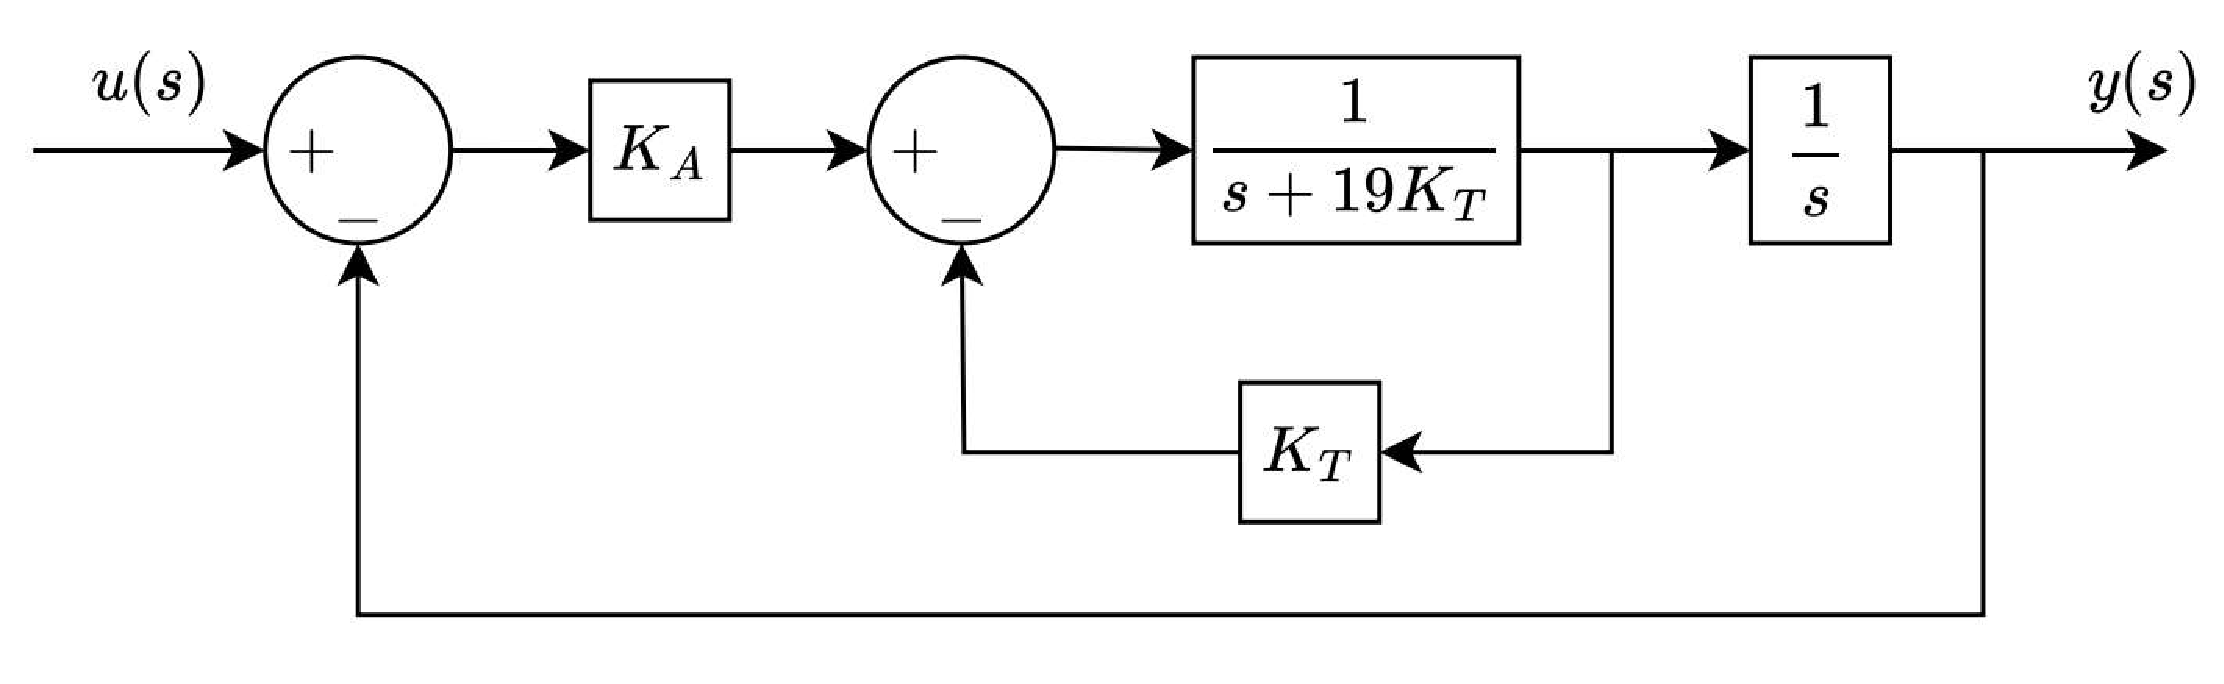
\includegraphics[width=0.5\textwidth]{Auxiliar_3_1}
        \captionof{figure}{Esquema del circuito}
    \end{center}

    %%%%%%%%%%%%%%%%%%%%%%%%%%%%
    \begin{solution}
        Se busca el obtener el voltaje $v_{sal}$, por lo tanto sera de utilidad considerar la equivalencia \textit{Thevenin - Norton} para el circuito, por lo tanto dividiendo por zonas:
        \begin{center}
            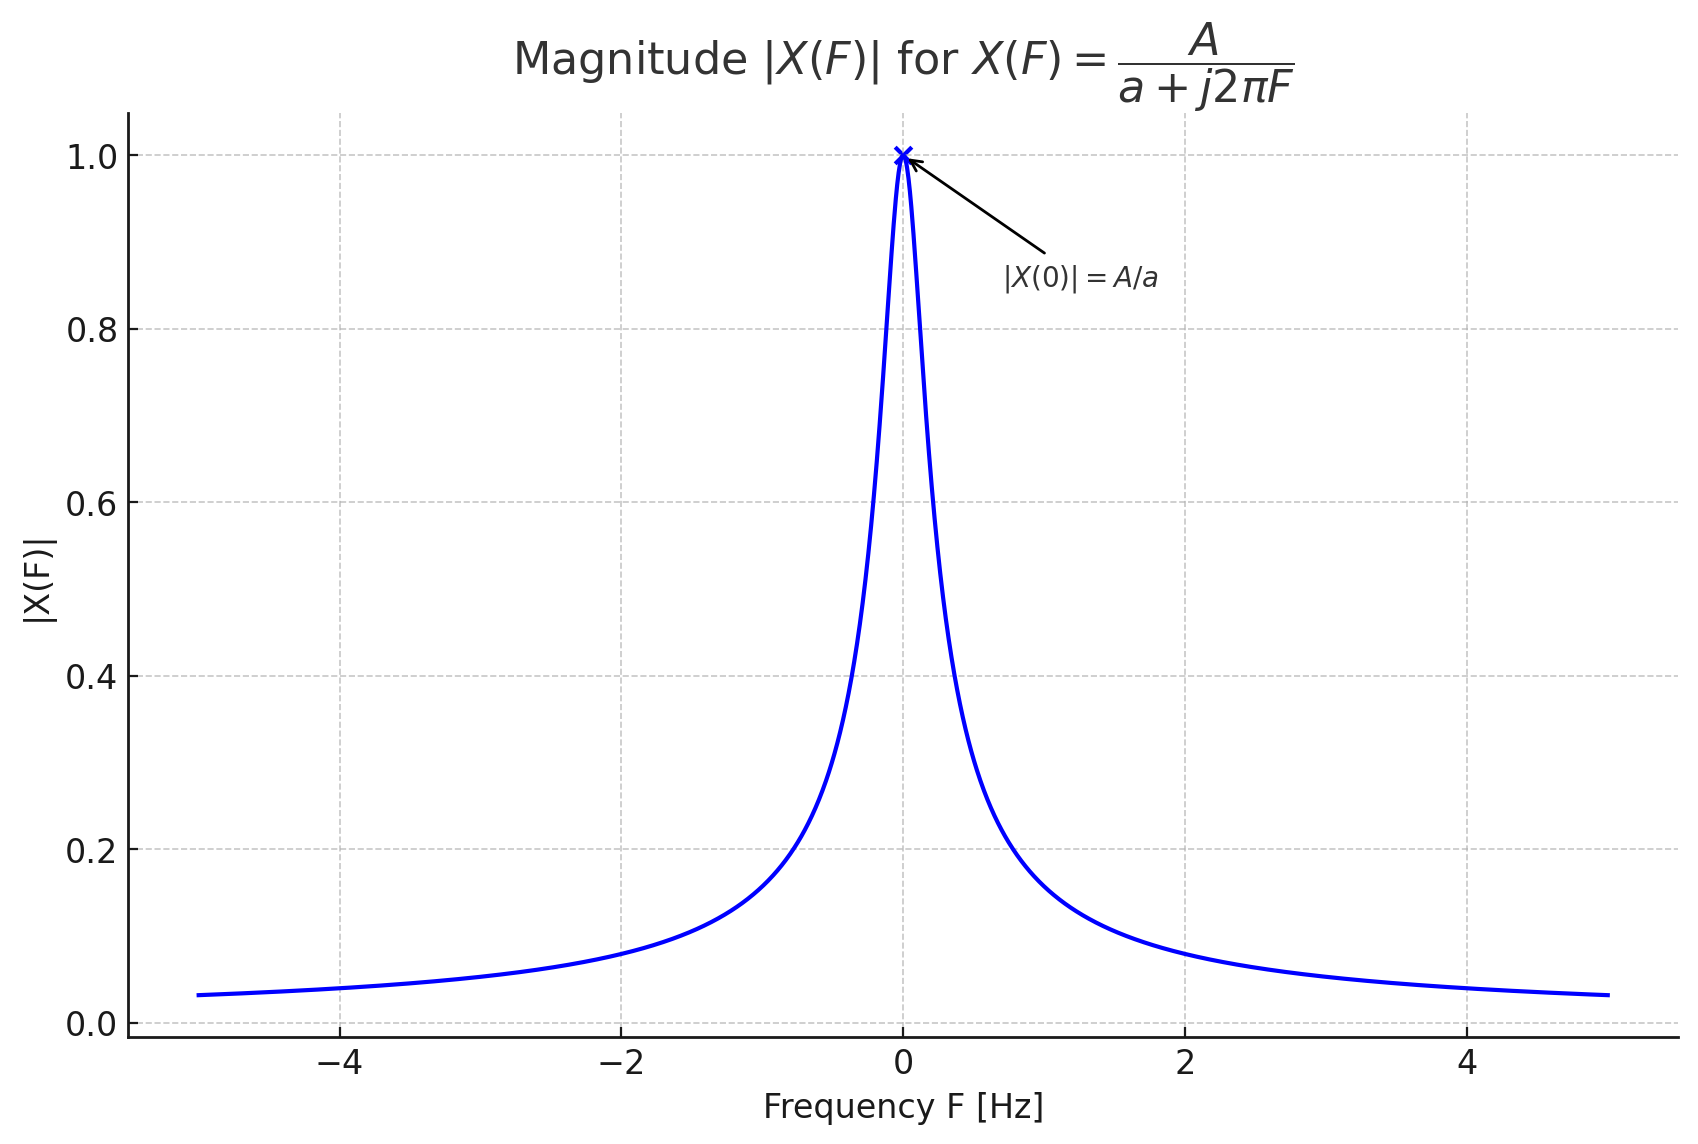
\includegraphics[width=0.5\textwidth]{Auxiliar_3_2}
            \captionof{figure}{Esquema del circuito}
        \end{center}
        Por lo tanto para la zona 1 tenemos que:
        \begin{center}
            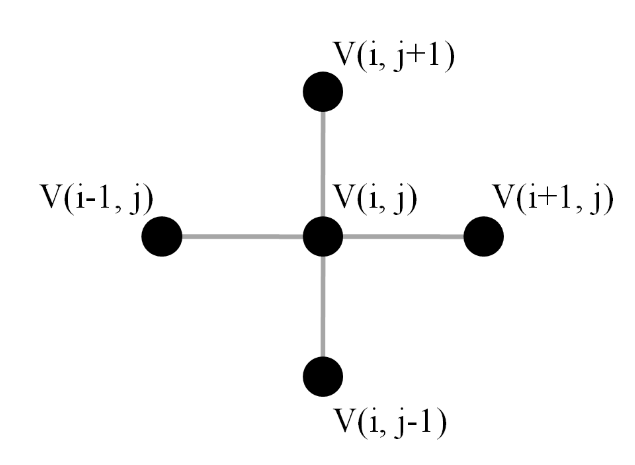
\includegraphics[width=0.3\textwidth]{Auxiliar_3_3}
            \captionof{figure}{Esquema del circuito}
        \end{center}
        Donde notamos que la resistencia de $6[\Omega]$ y la de $3[\Omega]$ se encuentran en paralelo, es decir:
        \begin{equation}
            R_{eq} = \frac{6[\Omega] \cdot 3[\Omega]}{6[\Omega] + 3[\Omega]} = 2[\Omega]
        \end{equation}
        Con lo que se obtiene que:
        \begin{center}
            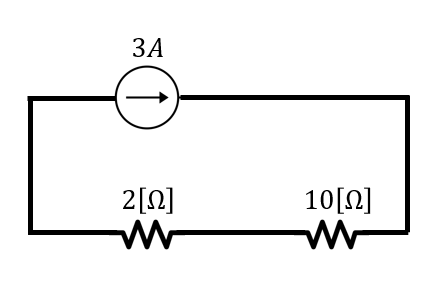
\includegraphics[width=0.3\textwidth]{Auxiliar_3_4}
            \captionof{figure}{Esquema del circuito}
        \end{center}
        Donde notamos que la resistencia equivalente de $2[\Omega]$ y la de $10[\Omega]$ se encuentran en serie, es decir:
        \begin{equation}
            R_{eq} = 2[\Omega] + 10[\Omega] = 12[\Omega]
        \end{equation}
        De esta manera podemos aplicar la equivalencia de Thevenin - Norton, por lo tanto se tiene que:
        \begin{center}
            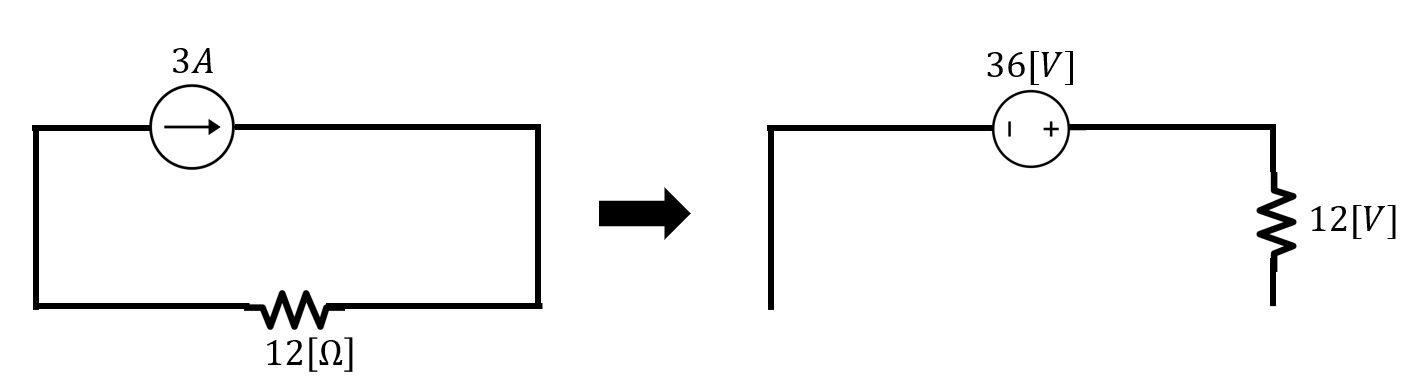
\includegraphics[width=0.6\textwidth]{Auxiliar_3_5}
            \captionof{figure}{Esquema del circuito}
        \end{center}
        Luego analogamente para la zona 2 tenemos que:
        \begin{center}
            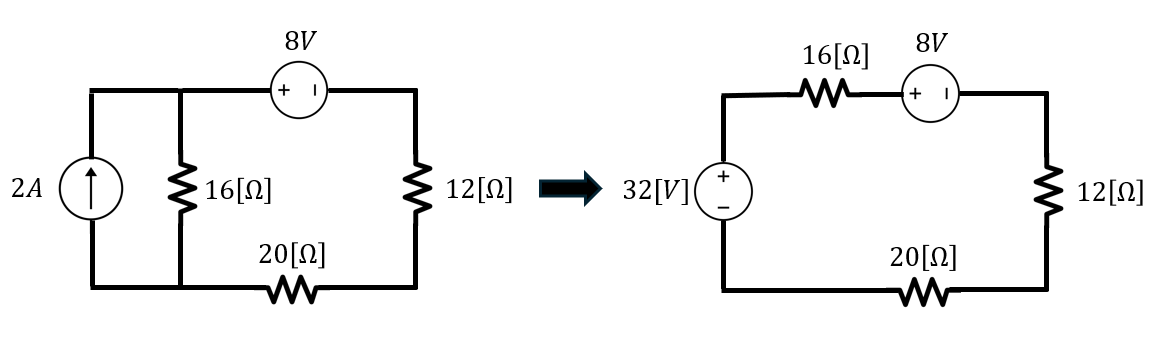
\includegraphics[width=0.6\textwidth]{Auxiliar_3_6}
            \captionof{figure}{Esquema del circuito}
        \end{center}
        De esta manera tenemos que las dos resistencias estan en serie por lo que:
        \begin{equation}
            R_{eq} = 16[\Omega] + 20[\Omega] = 36[\Omega]
        \end{equation} 
        Ademas tenemos dos resistencia en sentido opuestos, por lo que se restan dando como resultado:
        \begin{align}
            V_{eq} = 32[V] - 8[V] = 24[V]\\
        \end{align}
        Por lo que el esquema final vendra dado por:
        \begin{center}
            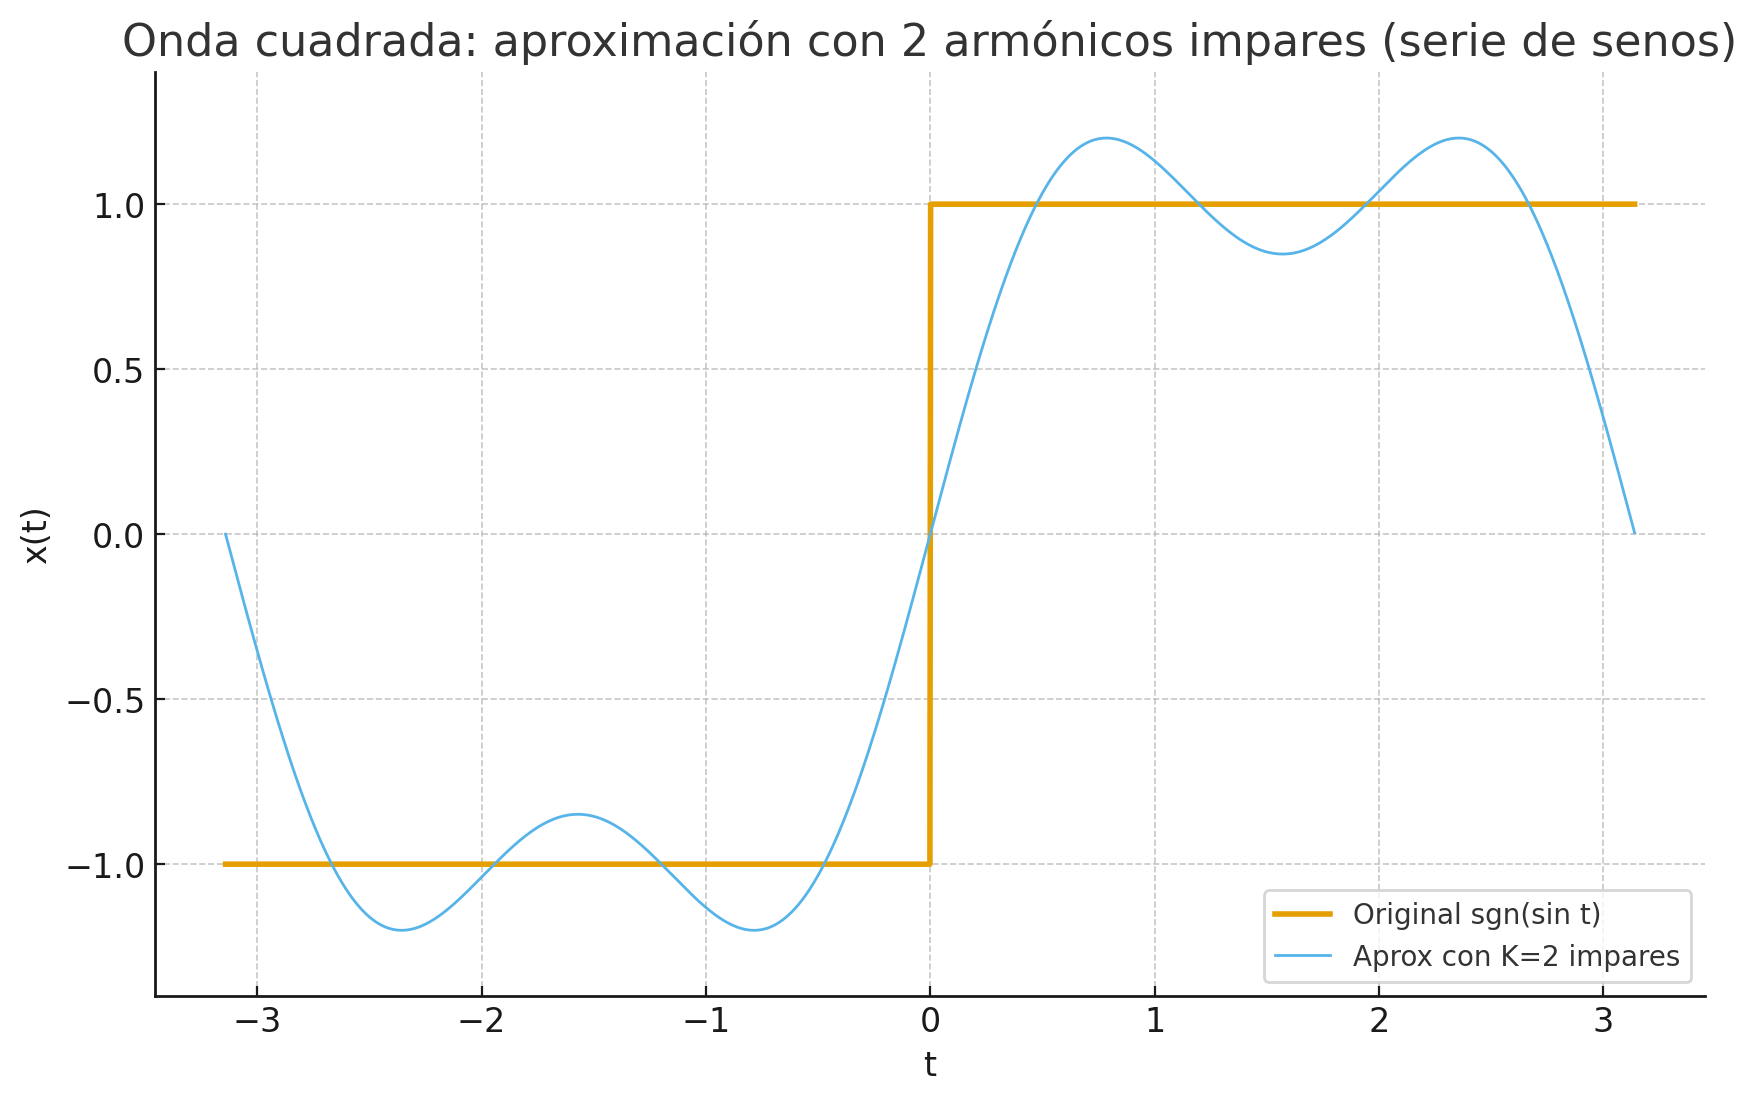
\includegraphics[width=0.4\textwidth]{Auxiliar_3_7}
            \captionof{figure}{Esquema del circuito}
        \end{center}
        Recordemos que esta zona se encuentra conectada al resto del circuito por lo que los voltajes 12$[\Omega]$ Y 36$[\Omega]$ no se encuentran ni en serie ni en paralelo, lo que podemos realizar por tanto es utilizar otra vez la equivalencia de Thevenin - Norton, por lo que se tiene que:
        \begin{center}
            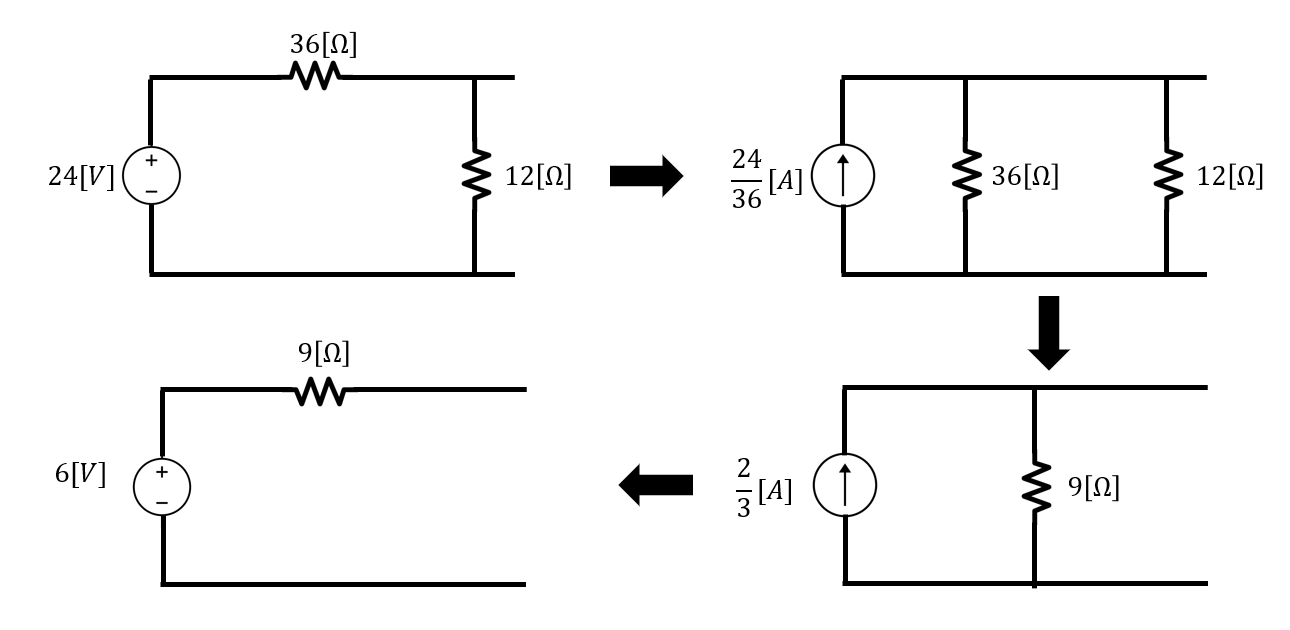
\includegraphics[width=0.6\textwidth]{Auxiliar_3_8}
            \captionof{figure}{Esquema del circuito}
        \end{center}
        De esta manera tenemos que el circuito original vendra dado por:
        \begin{center}
            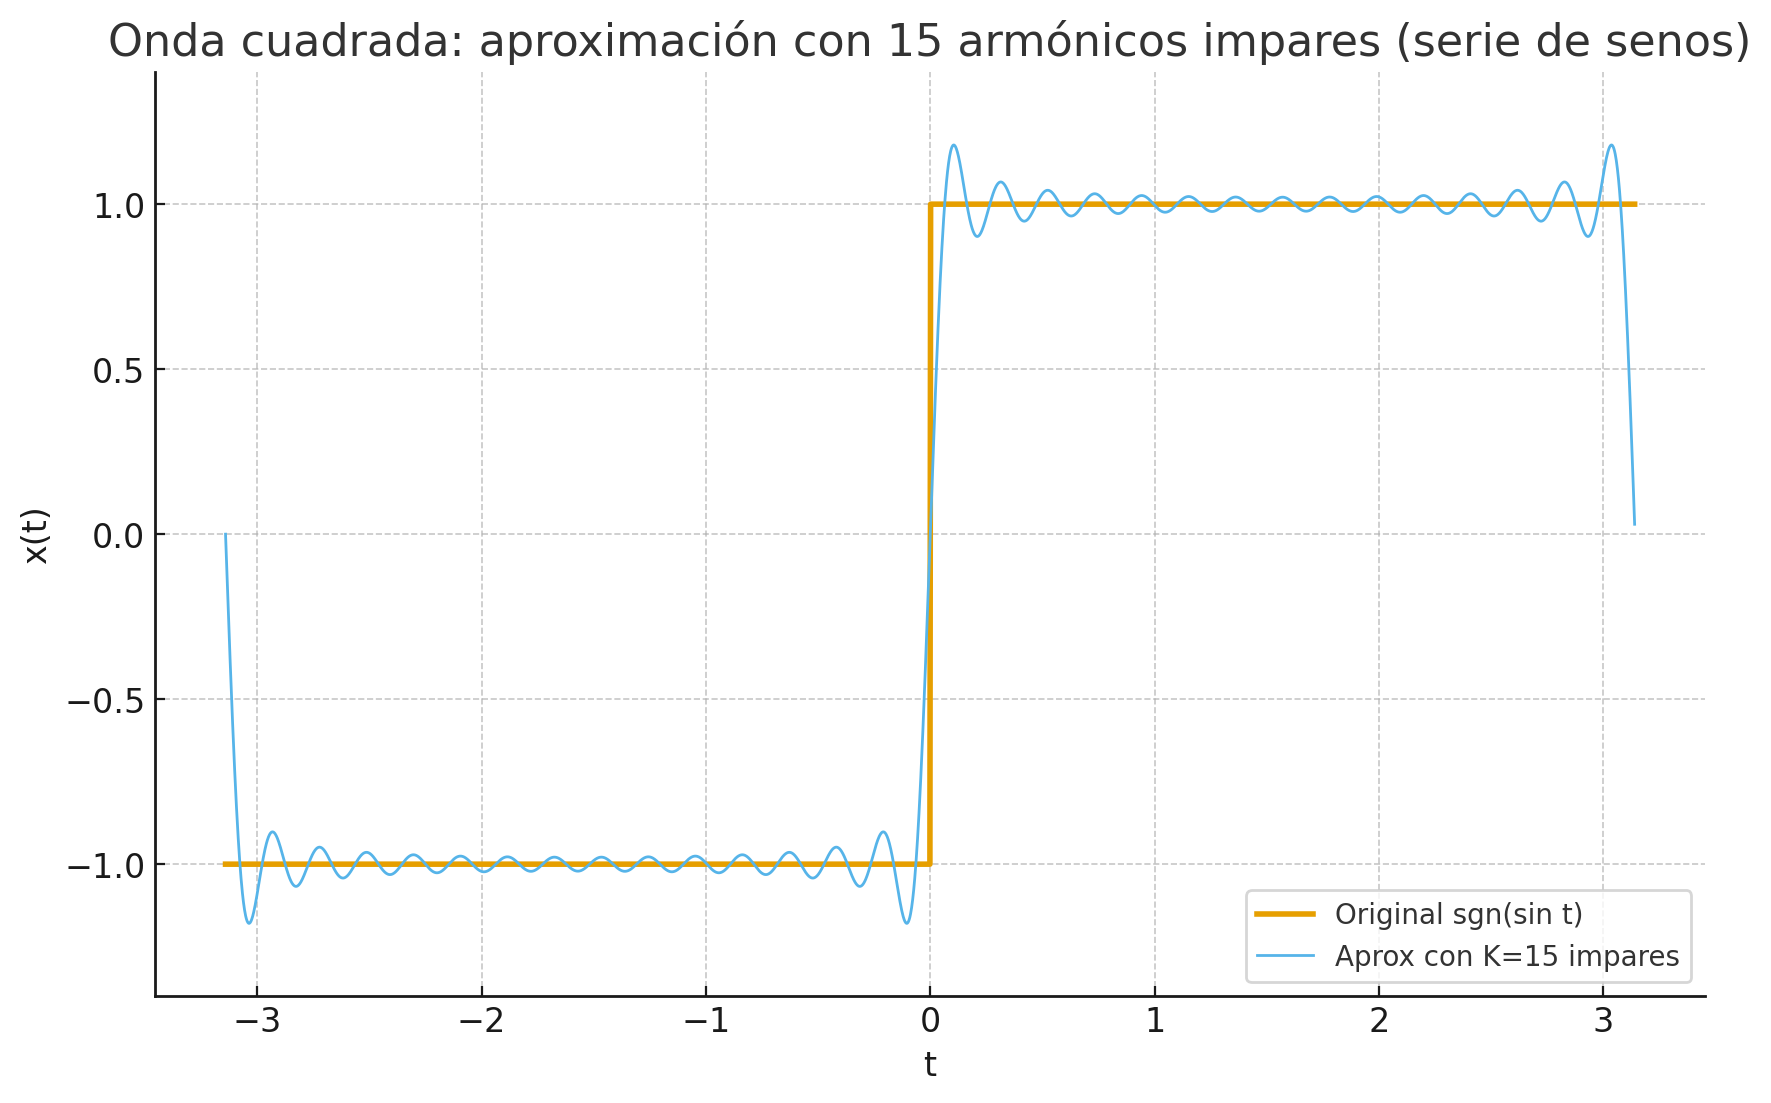
\includegraphics[width=0.4\textwidth]{Auxiliar_3_9}
            \captionof{figure}{Esquema del circuito}
        \end{center}
        Con lo que el circuito se simplifica de sobremanera, por lo que unicamente tenemos una malla dada por
        \begin{equation}
        -6 +9i - 36 + 12i + 7i - V_{sal}=0 
    \end{equation}:
    y dado que la corriente i es conocid,tenemos finalmente que el $v_{sal}$ sera:
        \begin{align}
            V_{sal} &= 6 + 9i - 36 + 12i + 7i \\
            &= -30 + 28i
        \end{align}
        De esta manera se obtiene el voltaje $v_{sal}$ en funcion de la corriente $i$.
    \end{solution}
    %%%%%%%%%%%%%%%%%%%%%%%%%%%
    \question  Sea el esquema visto en la figura  , obtenga la corriente $i_{R}$ en la resistencia $R= 1/6 [\Omega]$ 
    \begin{center}
        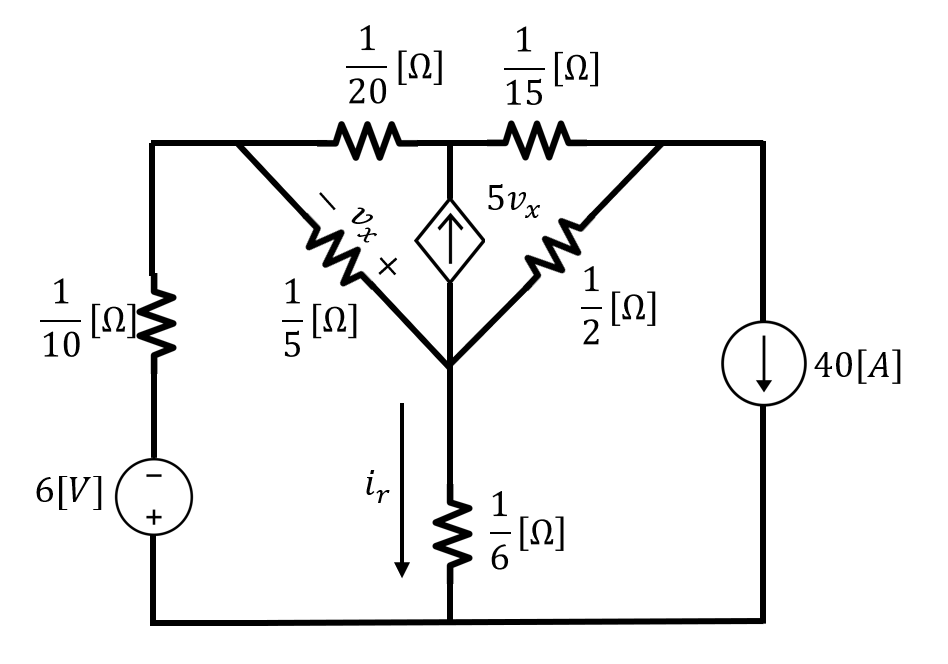
\includegraphics[width=0.5\textwidth]{Auxiliar_3_10}
        \captionof{figure}{Esquema del circuito}
    \end{center}
    %%%%%%%%%%%%%%%%%%%%%%%%%%%
    \begin{solution}
        Se resolvera mediante metodo de nodos, por lo tanto se plantea lo siguiente:
        \begin{center}
            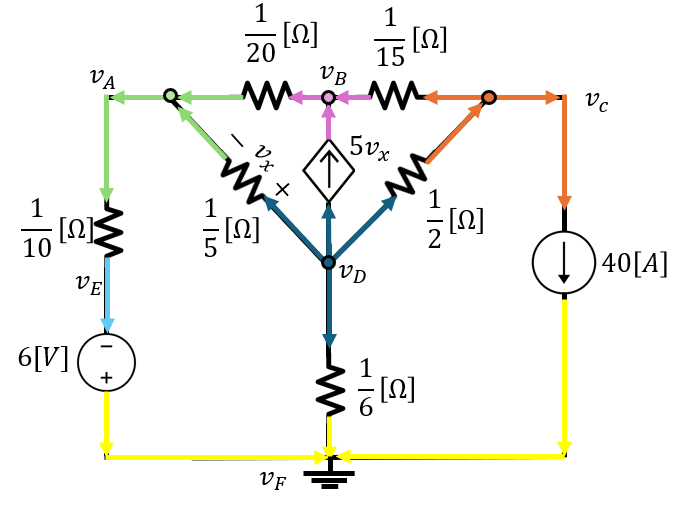
\includegraphics[width=0.5\textwidth]{Auxiliar_3_11}
            \captionof{figure}{Esquema del circuito}
        \end{center}
        Con lo es posible plantear las siguientes ecuaciones, teniendo en consideracion que $V_{F} = 0$ Y $V_{E}= -6[V]$,dada la eleccion de la tierra, luego:
        \begin{align}
            \text{Nodo A:} \quad & i_{20} + i_{5} = i_{10}\\
            & (V_{b} - V_{a})20 + (V_{D} - V_{a})5 = (V_{a} + 6)10\\
            \text{Nodo B:} \quad & i_{5v_{x}} + i_{15} = i_{20}\\
            & 5V_{x} + (V_{c} - V_{b})15 = (V_{b} - V_{a})20\\
            \text{Nodo C:} \quad & i_{2} =i_{15} + 40\\
            & (V_{D} - V_{c})2 = (V_{c} - V_{b})15 + 40\\
            \text{Nodo D:} \quad & i_{5} + i_{2} +i_{6} +i_{5v_{x}} = 0\\
            & (V_{D} - V_{a})5 + (V_{D} - V_{c})2 + 6v_{D} + 5V_{x} = 0\\
        \end{align}
        Pero tenemos que $V_{x} = V_{D} - V_{A}$, por tanto se tiene el siguiente sistema de ecuaciones:
        \begin{align}
            -35v_A + 20v_B + 5v_D &= 60 \\
            15v_A - 35v_B + 15v_C + 5v_D &= 0 \\
            15v_B - 17v_C + 2v_D &= 40 \\
            -10v_A - 2v_C + 18v_D &= 0
        \end{align}
        Con lo que despejando el sistema de ecuaciones tenemos que:
        \begin{align}
            v_A &= -7[V] \\
            v_B &= -8[V] \\
            v_C &= -10[V] \\
            v_D &= -5[V]
        \end{align}
        De esta manera tenemos que la corriente $i_R$ sera:
        \begin{align}
            i_R &= \frac{V_{D} - V_{F}}{\frac{1}{6}} \\
            &= \frac{-5 - 0}{\frac{1}{6}} \\
            &= -30[A]
        \end{align}
        Con lo que finalmente tenemos que la corriente $i_R$ es de $-30[A]$, lo que indica que la corriente fluye en sentido opuesto al planteado.
    \end{solution}
%%%%%%%%%%%%%%%%%%%%%%%%%%%

\question Considera el circuito de la figura 1 (a) donde $V_b$, $V_1$ y $V_2$ son fuentes de voltajes conocidos. En particular las últimas dos están referenciadas a tierra.
Se solicita entonces:
\begin{center}
    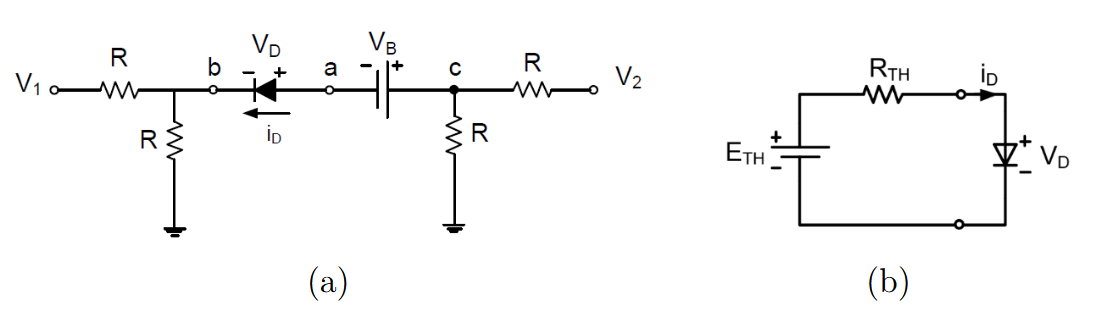
\includegraphics[width=0.7\textwidth]{Auxiliar_3_12}
    \captionof{figure}{Esquema del circuito}
\end{center}
\begin{enumerate}
    \item Encontrar el equivalente de Thevenin desde los terminales a-b para obtener el circuito equivalente de la figura 1 (b). 
    \item Encuentre las condiciones de $V_2$ tal que el diodo esté en estado ON/OFF. 
    \item Imponga $V_1 = 0 [V]$, $V_B = 1 [V]$. Si $V_2$ es la onda rectangular de la figura 2, encuentre y grafique el comportamiento del voltaje $V_C$ en función del tiempo. 
\end{enumerate}
\begin{center}
    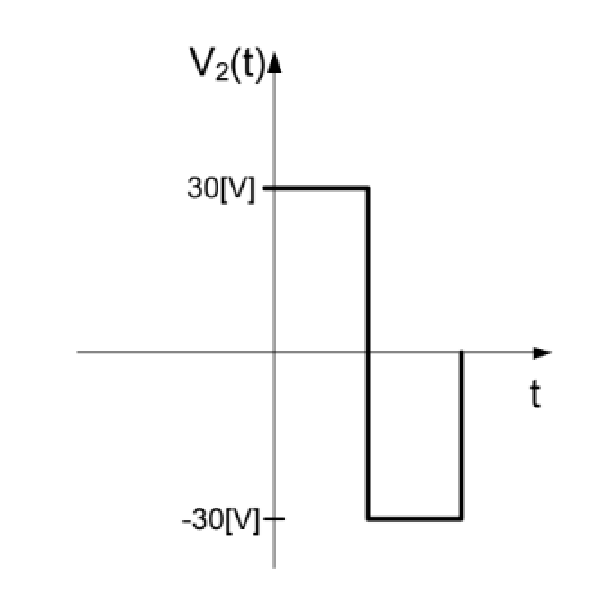
\includegraphics[width=0.3\textwidth]{Auxiliar_3_13}
    \captionof{figure}{Esquema del circuito}
\end{center}
%%%%%%%%%%%%%%%%%%%%%%%%%%%
\begin{solution}
    \begin{enumerate}
        \item Dado que se busca obtener el equivalente de Thevenin, primero se realizan unas reduccion con el fin de simplificar mas el circuito, es decir:
        \begin{center}
            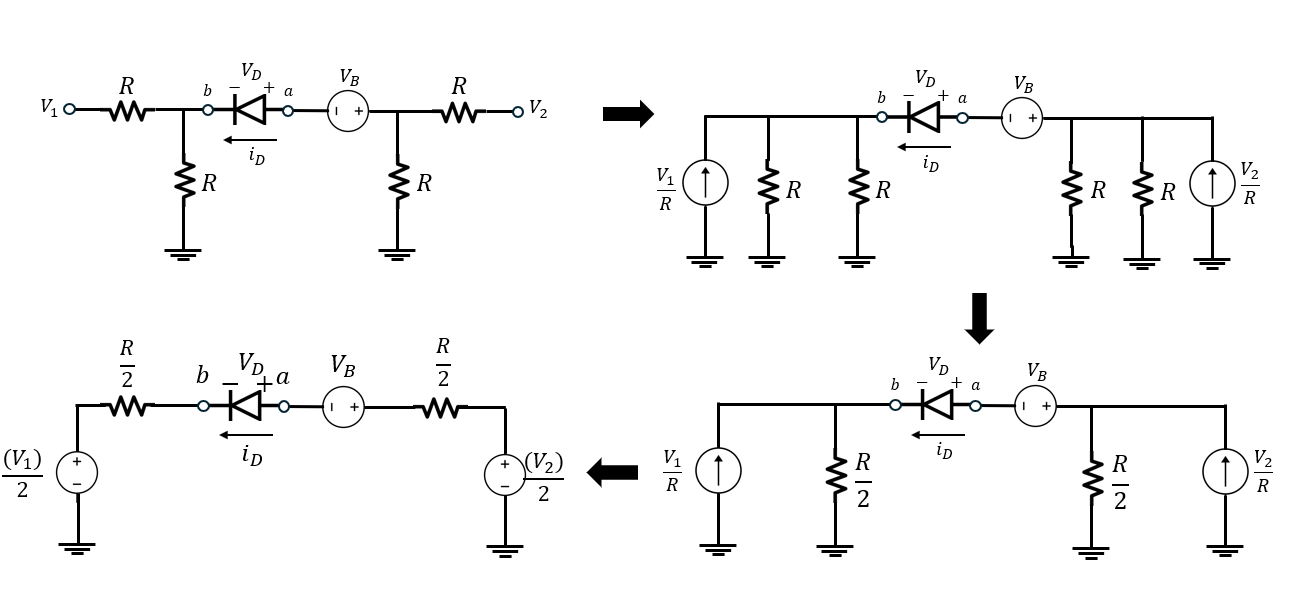
\includegraphics[width=0.8\textwidth]{Auxiliar_3_14}
            \captionof{figure}{Esquema del circuito}
        \end{center}
    Luego se busca obtener el voltaje de Thevenin y la resistencia de theve, para el primero debemos cortocircuitar las fuentes de voltaje y dejar abiertas las fuentes de corriente (En caso de existir), por lo que se tiene que:
    \begin{center}
        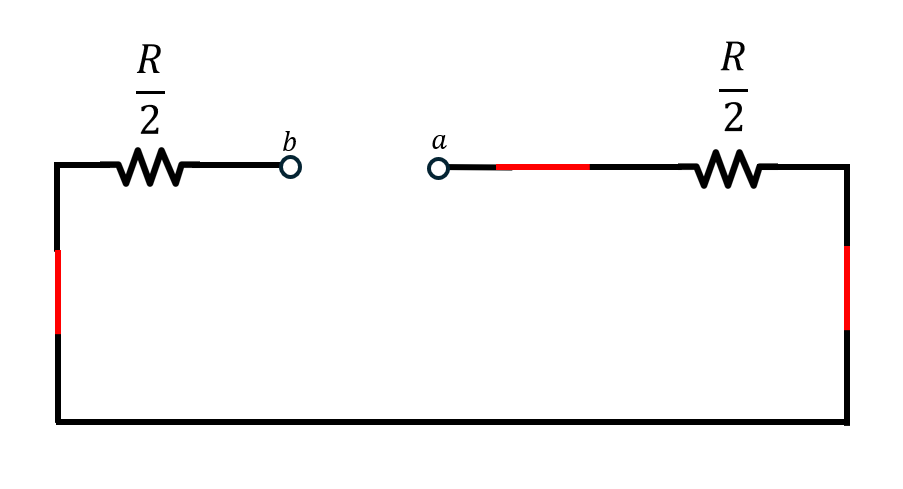
\includegraphics[width=0.35\textwidth]{Auxiliar_3_15}
        \captionof{figure}{Esquema del circuito}
    \end{center}
    Tenemos por tanto que la resistencia de Thevenin sera:
    \begin{equation}
        R_{th} = \frac{R}{2} + \frac{R}{2} = R
    \end{equation}
    Por otro lado tendremos que el voltaje de Thevenin sera:
    \begin{center}
        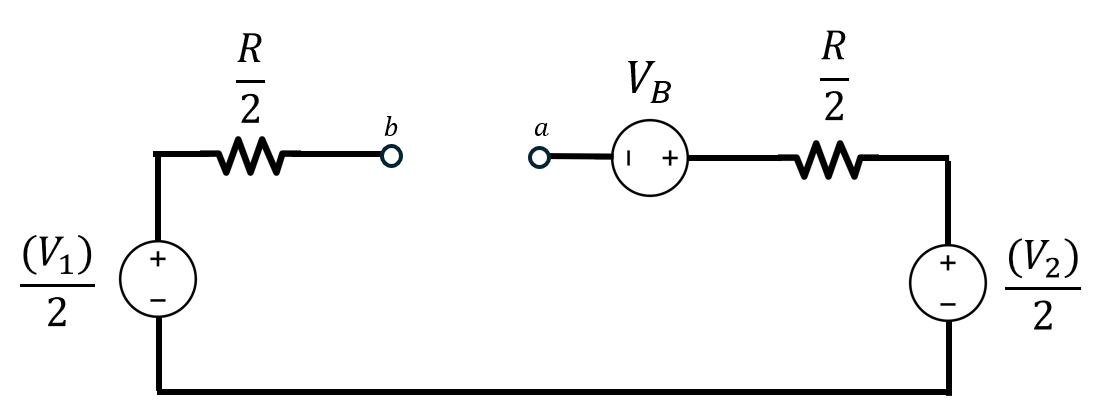
\includegraphics[width=0.45\textwidth]{Auxiliar_3_16}
        \captionof{figure}{Esquema del circuito}
    \end{center}
    De esta manera tenemos que el circuito vendra dado por una malla tal que:
    \begin{align}
        0 = \frac{-V_{1}}{2} + i\frac{R}{2} - V_{B} + i\frac{R}{2} + \frac{V_{2}}{2}-V_{th}\\
        v_{th}= \frac{V_{2}- v_{1}}{2} - V_{b}
    \end{align}
    Con lo que de esta manera tenemos que el sistema reducido corresopndera a :
    \begin{center}
        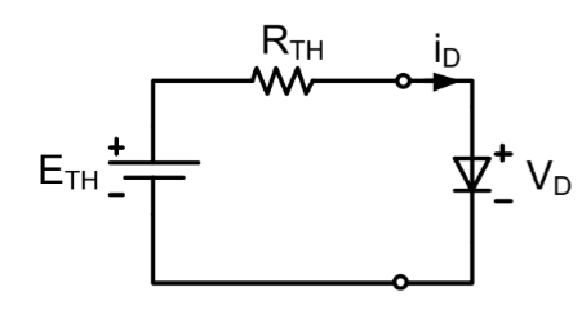
\includegraphics[width=0.3\textwidth]{Auxiliar_3_17}
        \captionof{figure}{Esquema del circuito}
    \end{center}
    obteniendo lo buscado.
    \item Se busca las condiciones de $V_2$ tal que el diodo se encuentre en estado ON/OFF, por lo que tenemos que dividir por casos:
    \begin{itemize}
        \item \textbf{Estado OFF:} En este caso tenemos que se debe cumplir que $I_{D} = 0$ y para esto se debe tener que $V_{D} < 0$ por lo tanto retomando la ecuacion anterior, se realiza una malla en el sistema reducido y por tanto:
        \begin{align}
            V_{th} + Ri_{D} +V_{D}&= 0\\
            \frac{V_{2}- V_{1}}{2} - V_{b} + Ri_{D} +V_{D}&= 0
        \end{align} 
        Pero sabemos que $I_{D}= 0 $ en el caso en que el diodo este en OFF y por lo tanto $V_{D} < 0 $:
        \begin{align}
            \frac{V_{2}- V_{1}}{2} - V_{b} +V_{D}= 0\\
            V_{D} = -\frac{V_{2}- V_{1}}{2} + V_{b}\\
        \end{align} 
        Dado que $V_{D} < 0$, despejando $v_{2}$ se tendra que:
        \begin{align}
            V_{2} &< V_{1} + 2V_{b}\\
        \end{align}
        \item \textbf{Estado ON:} En este caso tenemos que se debe cumplir que $I_{D} > 0$ y para esto se debe tener que $V_{D} = 0$ por lo tanto retomando la ecuacion anterior, se realiza una malla en el sistema reducido y por tanto:
        \begin{align}
            V_{th} + Ri_{D} +V_{D}&= 0\\
            \frac{V_{2}- V_{1}}{2} - V_{b} + Ri_{D} +V_{D}&= 0
        \end{align} 
        Se debe cumpli rque $Ri_{D} > 0 $ ademas que $V_{D} = 0$, por lo que se tiene que:
        \begin{equation}
            Ri_{D} = -\frac{V_{2}- V_{1}}{2} + V_{b} > 0 
        \end{equation}
        De esta manera se tiene que despejando $V_{2}$ se tendra que:
        \begin{align}
            V_{2} &> V_{1} + 2V_{b}\\
        \end{align}
    \end{itemize}
    Por lo que se determinan las condiciones de $V_2$ tal que el diodo esté en estado ON/OFF.
    \item Se impone $V_1 = 0 [V]$, $V_B = 1 [V]$, viendo el grafico tenemos que $V_{2}= 30$ inicialmente, por lo que en base a las desigualdades anteriores tenemos que:
    \begin{equation}
        2V_{b} + V_{1}= 2 
    \end{equation}
    Por lo que es mayor que $0$, por lo que el diodo se encuentra en estado ON, por lo que el voltaje $V_{C}$ sera:
\end{enumerate}
\end{solution}
%%%%%%%%%%%%%%%%%%%%%%%%%%%%%%
\question
    Para el circuito de la figura, calcule las corrientes de malla:
    \begin{center}
        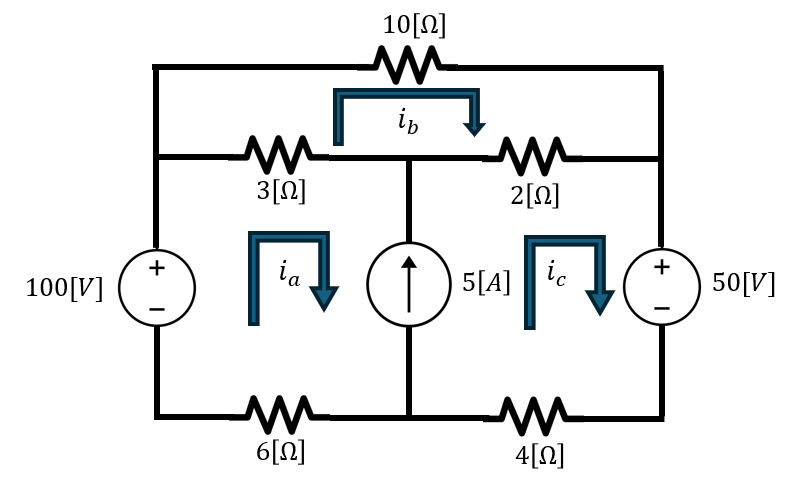
\includegraphics[width=0.6\textwidth]{Auxiliar_3_18}
        \captionof{figure}{Esquema del circuito}
    \end{center}
\end{questions}
\end{document}